% !BIB TS-program = biber

\RequirePackage[l2tabu,orthodox]{nag}

% TODO: decide if one-sided/two-sided
%\documentclass[headsepline,footsepline,footinclude=false,fontsize=11pt,paper=a4,listof=totoc,bibliography=totoc,BCOR=12mm,DIV=12]{scrbook} % two-sided
\documentclass[headsepline,footsepline,footinclude=false,oneside,fontsize=11pt,paper=a4,listof=totoc,bibliography=totoc]{scrbook} % one-sided

% TODO: change thesis information
\newcommand*{\getUniversity}{Technische Universität München}
\newcommand*{\getFaculty}{Informatics}
\newcommand*{\getDegree}{Informatics}
\newcommand*{\getSchool}{Computation, Information and Technology}
\newcommand*{\getTitle}{Design, Implementation and Test of a Python API for the sys-sage Library}
\newcommand*{\getTitleGer}{Design, Implementierung und Test einer Python API für die sys-sage Library}
\newcommand*{\getAuthor}{Jonathan Wieser}
\newcommand*{\getDoctype}{Bachelor's Thesis}
\newcommand*{\getSupervisor}{Prof. Dr. rer. nat. Martin Schulz}
\newcommand*{\getAdvisor}{Stepan Vanecek}
\newcommand*{\getKeywords}{keyword;another keyword;one more}
\newcommand*{\getSubmissionDate}{14.04.2025}
\newcommand*{\getSubmissionLocation}{Munich}

% TODO: change citation style in settings
\PassOptionsToPackage{table,svgnames,dvipsnames}{xcolor}

\usepackage[a-2u]{pdfx} % generate PDF/A: archival compliant, self-contained pdf
\usepackage[utf8]{inputenc}
\usepackage[T1]{fontenc}
\usepackage[sc]{mathpazo}
\usepackage[german,american]{babel}
\usepackage[autostyle]{csquotes}
\usepackage[%
  backend=biber,
  url=false,
  style=numeric,
  maxnames=4,
  minnames=3,
  maxbibnames=99,
  giveninits,
  uniquename=init]{biblatex} % TODO: adapt citation style
\usepackage{graphicx}
\usepackage{scrhack} % necessary for listings package
\usepackage{listings}
\usepackage{lstautogobble}
\usepackage{tikz}
\usepackage{pgfplots}
\usepackage{pgfplotstable}
\usepackage{booktabs}
\usepackage[final]{microtype}
\usepackage{caption}
\usepackage[printonlyused]{acronym}
\usepackage{ifthen}
\usepackage{svg}



\hypersetup{hidelinks} % removes colored boxes around references and links

% for fachschaft_print.pdf
\makeatletter
\if@twoside
	\typeout{TUM-Dev LaTeX-Thesis-Template: twoside}
\else
	\typeout{TUM-Dev LaTeX-Thesis-Template: oneside}
\fi
\makeatother

\addto\extrasamerican{
	\def\lstnumberautorefname{Line}
	\def\chapterautorefname{Chapter}
	\def\sectionautorefname{Section}
	\def\subsectionautorefname{Subsection}
	\def\subsubsectionautorefname{Subsubsection}
}

\addto\extrasngerman{
	\def\lstnumberautorefname{Zeile}
}

% Themes
\ifthenelse{\equal{\detokenize{dark}}{\jobname}}{%
  % Dark theme
  \newcommand{\bg}{black} % background
  \newcommand{\fg}{white} % foreground
  \usepackage[pagecolor=\bg]{pagecolor}
  \color{\fg}
}{%
  % Light theme
  \newcommand{\bg}{white} % background
  \newcommand{\fg}{black} % foreground
}

\bibliography{bibliography}

\setkomafont{disposition}{\normalfont\bfseries} % use serif font for headings
\linespread{1.05} % adjust line spread for mathpazo font

% Add table of contents to PDF bookmarks
\BeforeTOCHead[toc]{{\cleardoublepage\pdfbookmark[0]{\contentsname}{toc}}}

% Define TUM corporate design colors
% Taken from http://portal.mytum.de/corporatedesign/index_print/vorlagen/index_farben
\definecolor{TUMBlue}{HTML}{0065BD}
\definecolor{TUMSecondaryBlue}{HTML}{005293}
\definecolor{TUMSecondaryBlue2}{HTML}{003359}
\definecolor{TUMBlack}{HTML}{000000}
\definecolor{TUMWhite}{HTML}{FFFFFF}
\definecolor{TUMDarkGray}{HTML}{333333}
\definecolor{TUMGray}{HTML}{808080}
\definecolor{TUMLightGray}{HTML}{CCCCC6}
\definecolor{TUMAccentGray}{HTML}{DAD7CB}
\definecolor{TUMAccentOrange}{HTML}{E37222}
\definecolor{TUMAccentGreen}{HTML}{A2AD00}
\definecolor{TUMAccentLightBlue}{HTML}{98C6EA}
\definecolor{TUMAccentBlue}{HTML}{64A0C8}

% Settings for pgfplots
\pgfplotsset{compat=newest}
\pgfplotsset{
  % For available color names, see http://www.latextemplates.com/svgnames-colors
  cycle list={TUMBlue\\TUMAccentOrange\\TUMAccentGreen\\TUMSecondaryBlue2\\TUMDarkGray\\},
}

% Settings for lstlistings
\lstset{%
  basicstyle=\ttfamily,
  columns=fullflexible,
  autogobble,
  keywordstyle=\bfseries\color{TUMBlue},
  stringstyle=\color{TUMAccentGreen},
  captionpos=b
}


\begin{document}

% Set page numbering to avoid "destination with the same identifier has been already used" warning for cover page.
% (see https://en.wikibooks.org/wiki/LaTeX/Hyperlinks#Problems_with_Links_and_Pages).
\pagenumbering{alph}
\input{pages/cover}

\frontmatter{}

\input{pages/title}
\input{pages/disclaimer}
%\input{pages/acknowledgments} 
\chapter{\abstractname}

\noindent High-Performance Computing (HPC) continues to be a prominent field, characterized by increasingly intricate topologies and the growing integration of accelerators such as GPUs. In such complex systems, analyzing resource allocation and system states is crucial, encompassing both static infrastructure and dynamic runtime behavior to identify bottlenecks and adapt to system changes. While existing tools address static and dynamic analysis separately, sys-sage uniquely combines these capabilities, offering a broad spectrum of functions to examine components and their interconnections. Its architecture allows users to tailor and extend functionalities to specific use cases, albeit requiring C++ proficiency.   

To enhance usability and facilitate rapid prototyping for a wider audience, particularly those seeking an intuitive way to interact with sys-sage without extensive compilation, this work focuses on providing a Python interface. Python, a familiar language with a relatively gentle learning curve, is well-suited for prototyping and extending existing libraries. We analyze and compare the usability and performance characteristics of different technologies for achieving this Python binding, ultimately selecting and implementing a suitable solution. Furthermore, we introduce a new feature to the core sys-sage library in C++: XML import functionality. Comprehensive benchmarks are conducted to quantify the performance difference between the resulting Python interface and the native C++ implementation. The thesis concludes with a discussion of future work, including the integration of modified destructors within the sys-sage library to improve memory management and simplify the user experience.   



\microtypesetup{protrusion=false}
\tableofcontents{}
\microtypesetup{protrusion=true}

\mainmatter{}

% !TeX root = ../main.tex
% Add the above to each chapter to make compiling the PDF easier in some editors.

\chapter{Introduction}\label{chapter:introduction}
\section{Introduction to Sys-Sage Library}

High-Performance Computing (HPC) systems have undergone significant transformations, becoming increasingly complex. This complexity arises from the integration of various components, particularly the growing reliance on multi-core processors and \ac{GPU}s. As modern architectures evolve, understanding system behavior becomes more challenging, necessitating more sophisticated analysis tools.

Several approaches exist for analyzing system architectures, with one of the most commonly used tools being \texttt{hwloc}. This tool facilitates the construction of hardware topologies, mapping essential building blocks such as cores, caches, and \ac{NUMA} nodes. While \texttt{hwloc} provides fundamental insights into system topology and application scheduling, it is limited to \ac{CPU}-based static analysis.

However, contemporary architectures introduce dynamic resource allocation and isolation, rendering static analysis insufficient for comprehensive system evaluation. Consequently, dynamic analysis becomes increasingly valuable in modern computing environments. Given the growing dynamism of \ac{HPC} systems, a unified tool that consolidates the advantages of existing solutions while incorporating real-time hardware and resource utilization changes would be highly beneficial.

The \texttt{Sys-Sage} library addresses this need by offering a unified \ac{API} for accessing the state of modern architectures. As an \ac{open-source} solution, \texttt{Sys-Sage} is highly adaptable and supports the integration of diverse datasets, such as \ac{GPU} benchmarks and power efficiency metrics, enabling a comprehensive understanding of system performance. It constructs an internal representation of hardware topology alongside data paths, allowing for both \textbf{export} and, in future iterations, \textbf{import} capabilities to facilitate data storage and retrieval.

\section{Scope of This Work}

Currently, \texttt{Sys-Sage} provides support exclusively for \ac{C++}, limiting its accessibility to a broader audience. Meanwhile, \ac{Python} has emerged as the most widely used programming language, surpassing JavaScript with \textbf{16.925\%} of all GitHub projects developed in \ac{Python}\parencite{python-github-stats}. Given its widespread adoption, introducing a \ac{Python} \ac{API} for \texttt{Sys-Sage} would significantly enhance usability, enabling a larger community to leverage its capabilities.

The objective of this work is to develop a \ac{Python} interface for \texttt{Sys-Sage} while preserving the performance advantages of the underlying \ac{C++} implementation. This will be achieved by binding essential \ac{C++} library functions, allowing users to compile the code once and execute scripts efficiently with the compiled runtime.

The \ac{Python} \ac{API} must meet the following key requirements:
\begin{itemize}
    \item \textbf{Ease of installation} – Users should be able to set up the library with minimal effort.
    \item \textbf{User-friendliness} – The \ac{API} should offer an intuitive interface for seamless integration into \ac{Python}-based workflows.
    \item \textbf{High performance} – The binding should maintain the speed and efficiency of the original \ac{C++} implementation.
\end{itemize}

By achieving these objectives, this project will bridge the gap between \texttt{Sys-Sage}'s powerful analysis capabilities and the growing \ac{Python} developer community, fostering broader adoption and enhanced system analysis in \ac{HPC} environments.

\subsection{Acronyms}

Acronyms must be added in \texttt{main.tex} and are referenced using macros. The first occurrence is automatically replaced with the long version of the acronym, while all subsequent usages use the abbreviation.

For example: \texttt{\textbackslash ac\{TUM\}, \textbackslash ac\{TUM\}} $\Rightarrow$ \ac{TUM}, \ac{TUM}.

For more details, see the documentation of the \texttt{acronym} package\footnote{\url{https://ctan.org/pkg/acronym}}.

% \printbibliography

\section{Section}
Citation test~\parencite{latex}.


Acronyms must be added in \texttt{main.tex} and are referenced using macros. The first occurrence is automatically replaced with the long version of the acronym, while all subsequent usages use the abbreviation.

E.g. \texttt{\textbackslash ac\{TUM\}, \textbackslash ac\{TUM\}} $\Rightarrow$ \ac{TUM}, \ac{TUM}

For more details, see the documentation of the \texttt{acronym} package\footnote{\url{https://ctan.org/pkg/acronym}}.
\subsection{Subsection}

See~\autoref{tab:sample}, \autoref{fig:sample-drawing}, \autoref{fig:sample-plot}, \autoref{fig:sample-listing}.

\begin{table}[htpb]
  \caption[Example table]{An example for a simple table.}\label{tab:sample}
  \centering
  \begin{tabular}{l l l l}
    \toprule
      A & B & C & D \\
    \midrule
      1 & 2 & 1 & 2 \\
      2 & 3 & 2 & 3 \\
    \bottomrule
  \end{tabular}
\end{table}

\begin{figure}[htpb]
  \centering
  % This should probably go into a file in figures/
  \begin{tikzpicture}[node distance=3cm]
    \node (R0) {$R_1$};
    \node (R1) [right of=R0] {$R_2$};
    \node (R2) [below of=R1] {$R_4$};
    \node (R3) [below of=R0] {$R_3$};
    \node (R4) [right of=R1] {$R_5$};

    \path[every node]
      (R0) edge (R1)
      (R0) edge (R3)
      (R3) edge (R2)
      (R2) edge (R1)
      (R1) edge (R4);
  \end{tikzpicture}
  \caption[Example drawing]{An example for a simple drawing.}\label{fig:sample-drawing}
\end{figure}

\begin{figure}[htpb]
  \centering

  \pgfplotstableset{col sep=&, row sep=\\}
  % This should probably go into a file in data/
  \pgfplotstableread{
    a & b    \\
    1 & 1000 \\
    2 & 1500 \\
    3 & 1600 \\
  }\exampleA
  \pgfplotstableread{
    a & b    \\
    1 & 1200 \\
    2 & 800 \\
    3 & 1400 \\
  }\exampleB
  % This should probably go into a file in figures/
  \begin{tikzpicture}
    \begin{axis}[
        ymin=0,
        legend style={legend pos=south east},
        grid,
        thick,
        ylabel=Y,
        xlabel=X
      ]
      \addplot table[x=a, y=b]{\exampleA};
      \addlegendimage{empty legend}
      \addlegendentry{Example A}
      \addplot table[x=a, y=b]{\exampleB};
      \addlegendentry{Example B}
    \end{axis}
  \end{tikzpicture}
  \caption[Example plot]{An example for a simple plot.}\label{fig:sample-plot}
\end{figure}

\begin{figure}[htpb]
  \centering
  \begin{tabular}{c}
  \begin{lstlisting}[language=SQL]
    SELECT * FROM table WHERE tbl.str = "str"
  \end{lstlisting}
  \end{tabular}
  \caption[Example listing]{An example for a source code listing.}\label{fig:sample-listing}
\end{figure}

\begin{figure}[htpb]
  \centering
  \includegraphics[width=\textwidth]{/home/jonjonjon/Thesis Tex/tum-thesis-latex/figures/pybind_schema.png}
  \caption[Example image]{An example for a simple image.}\label{fig:sample-image}
\end{figure}


\begin{figure}[hptb]
    \centering
  
    \pgfplotstableset{col sep=&, row sep=\\}
    \pgfplotstableread{
      x & swig & pybind11 \\
      10 & 0.831514591 & 1.058577497 \\
      20 & 1.127118936 & 1.471500208 \\
      30 & 1.4772158 & 1.761273233 \\
      40 & 1.736514494 & 2.126912437 \\
      50 & 2.025210358 & 2.46362231 \\
      60 & 2.214553424 & 2.804167879 \\
      70 & 2.603474917 & 3.326882148 \\
      80 & 2.877264073 & 3.673826322 \\
      90 & 3.352056939 & 3.967651672 \\
      100 & 3.392421572 & 4.391185498 \\
      110 & 3.703171002 & 4.916812021 \\
      120 & 4.275075549 & 5.214867283 \\
      130 & 5.214835618 & 5.347268902 \\
      140 & 6.241614607 & 5.945904962 \\
      150 & 6.595369415 & 6.519765277 \\
      160 & 6.967670258 & 7.11302645 \\
      170 & 7.165744065 & 7.452702384 \\
      180 & 7.80374477 & 7.193507064 \\
      190 & 8.358989104 & 7.662745811 \\
      200 & 8.92708868 & 7.899299085 \\
      210 & 9.175657786 & 8.070269308 \\
      220 & 9.27380257 & 8.513974392 \\
      230 & 9.771330559 & 8.768865073 \\
      240 & 10.07812149 & 8.980851734 \\
      250 & 10.57007511 & 9.686946998 \\
      260 & 10.93630689 & 9.962699361 \\
      270 & 11.02586082 & 10.96497769 \\
      280 & 11.80790557 & 10.70239503 \\
      290 & 12.17019807 & 11.02871699 \\
      300 & 12.6979764 & 11.43657468 \\
    }\data
  
    \begin{tikzpicture}
      \begin{axis}[
          ymin=0,
          ymax=20,
          legend style={legend pos=north west},
          grid,
          thick,
          ylabel=Time (seconds),
          xlabel=Hierarchy depth
        ]
        \addplot+[mark=none] table[x=x, y=swig]{\data};
        \addlegendentry{SWIG -O3, shared-pointers}
        \addplot+[mark=none] table[x=x, y=pybind11]{\data};
        \addlegendentry{PyBind11 -O3, shared-pointers}
      \end{axis}
    \end{tikzpicture}
    \caption[Plot of SWIG and PyBind11 with shared-pointers]{A plot comparing the performance of SWIG and PyBind11 with optimization flag -O3 and shared-pointers.}\label{fig:swig-pybind11-shared-pointers-plot}
  \end{figure}

\chapter{Terms and Definitions}\label{chapter:terms_and_definition}

\section{sys-sage Specific Terms}

To understand how \texttt{sys-sage} operates, it is essential to define its core concepts. \texttt{sys-sage} is designed with a modular structure, allowing for high adaptability through various compilation options that enable different functionalities. The system is primarily composed of components, data paths and their attributes, along with parsers and external interfaces, each serving a distinct role in modeling and analyzing complex hardware architectures.

\subsection{Components }

At the heart of \texttt{sys-sage} lies the concept of components, which represent various elements of a high-performance computing (\ac{HPC}) system. The most fundamental component is simply referred to as \texttt{Component}, a generic type that serves as the base class for all other component types. Every component inherits essential attributes such as \texttt{name}, \texttt{id}, and \texttt{type}, ensuring consistency across the system. \cite[see Component]{sys-sage-docu}

A key component type is \texttt{Topology}, which defines the root of an \ac{HPC} system. However, \texttt{sys-sage} allows any component to act as the root, offering flexibility in system representation. The \texttt{Node} component represents a computing node within an \ac{HPC} system and provides specific functions such as \texttt{RefreshCpuCoreFrequency()}, if \texttt{Proc\_Cpu} is enabled. This functions dynamically updates CPU frequencies. If the \texttt{Intel\_Pqos} extension is enabled, an additional function, \texttt{UpdateL3CATCoreCOS()}, becomes available, offering more control over cache allocation. \cite[see Topology, Node]{sys-sage-docu}

Memory is another crucial component in the system, represented by the \texttt{Memory} class. This component models various types of memory, with attributes such as \texttt{size}, which can be adjusted, and \texttt{volatility}, which remains static. For systems incorporating \texttt{NVIDIA MIG} technology, the memory component can retrieve the \texttt{MIGSize} of a \ac{GPU} memory partition. \cite[see Memory]{sys-sage-docu}

Similarly, the \texttt{Chip} component represents any type of processing unit, including CPUs, GPUs, and accelerators. It includes attributes such as \texttt{vendor}, \texttt{model}, and \texttt{chip-type}. When \texttt{NVIDIA MIG} is enabled, additional functionalities such as \texttt{UpdateMIGSettings()}, \texttt{GetMIGNumSMs()}, and \texttt{GetMIGNumCores()} provide extended configurability. \cite[see Chip]{sys-sage-docu}

To allow for hierarchical organization, \texttt{sys-sage} introduces the \texttt{Subdivision} component, which enables user-defined groupings within the system. A specialized subclass of \texttt{Subdivision} is \texttt{NUMA} (Non-Uniform Memory Access), which models memory locality and allows for adjustable memory sizes. \cite[see Subdivision, NUMA]{sys-sage-docu}  

Another critical component is the \texttt{Cache}, which represents cache memory within a system. It allows users to specify cache level, associativity ways, and cache-line size, determining how memory addresses map to cache lines. If \texttt{NVIDIA MIG} is enabled, the function \texttt{GetMIGSize()} becomes available, providing additional insights into GPU memory partitioning. \cite[see Cache]{sys-sage-docu}

At the processing level, the \texttt{Core} component models individual cores in CPUs or GPU streaming multiprocessors, with frequency attributes that can be both retrieved and modified. In addition, the \texttt{Thread} component represents hardware threads rather than software threads. While it also has a frequency attribute, this can only be read, not modified. If the \texttt{Intel\_Pqos} extension is enabled, the function \texttt{GetCATAwareL3Size()} provides additional cache-related information. \cite[see Core, Thread]{sys-sage-docu}

Ther are not only child-parent relationships. \texttt{sys-sage} also supports datapaths to connect arbitrary components.

\subsection{Datapaths}

In addition to components, \texttt{sys-sage} models interconnections within an \ac{HPC} system using datapaths. A datapath defines a link between two components, with each path having a well-defined source and target. While each component can have multiple data paths, individual data paths are unidirectional by default. However, bidirectional data paths can also be modeled, in which case they are stored twice — once as source and once as target. \cite[see Data Path]{sys-sage-docu}

Two primary attributes define data paths: \texttt{latency} and \texttt{bandwidth}, which are included by default. However, additional attributes can be incorporated depending on the specific use case, including parameters related to data transfer efficiency, system performance, and power consumption. These attributes allow data paths to accurately represent dynamic system behavior and adapt to changing configurations.\cite[see Data Path]{sys-sage-docu}

Datapaths share the same mechanism for additional attributes as Components, where the user has the option to add custom attributes.

\subsection{Attributes}

Both \texttt{Component} and \texttt{Datapath} classes contain a set of predefined attributes such as \texttt{id} and \texttt{name} or \texttt{orientation} and \texttt{bandwidth} respectively. However, \texttt{sys-sage} also allows users to define custom attributes through a flexible key-value mapping system. This feature enables components to store additional metadata, such as frequency history, while data paths can incorporate attributes related to power consumption or other performance characteristics.\cite[see Component, Datapath]{sys-sage-docu}
\smallskip

Now that we showed the essential parts to build a system topology, we will take a closer look at parsers and external interfaces, that help to build and feed the internal representation with data.

\subsection{Parsers}

To facilitate system analysis, \texttt{sys-sage} provides various parsers that allow the integration of external data sources. Supported parsers include \texttt{Caps\_Numa\_Benchmark}, \texttt{cccbench}, \texttt{hwloc}, and \texttt{mt4g}. These parsers enable the system to read relevant data and construct an internal representation of the hardware topology, making \texttt{sys-sage} a powerful tool for performance analysis and resource management.\cite[see Data Parsers Documentation]{sys-sage-docu}

\smallskip
Parsers play a important role in static analysis, but to use \texttt{sys-sage}'s dynamic features, the user can also integrate external interfaces.

\subsection{External Interfaces}

As menitioned in the Components section, some functions depend on external interfaces. These include \texttt{Intel\_Pqos}, \texttt{NVIDIA\_MIG}, and \texttt{Proc\_Cpuinfo}. They allow \texttt{sys-sage} to dynamically collect and analyze hardware performance data. However these interfaces are only available for systems, that have access to the respective technologies.\cite{sys-sage-docu}

We now have a overview of \texttt{sys-sage} and what role each of the main parts play. In order to grasp the potential challenges for binding the \texttt{sys-sage} library to Python, we will discuss the key differences between C++ and Python.

\section{Differences Between C++ and Python}

While \texttt{sys-sage} is implemented in C++, Python has emerged as one of the most popular programming languages, surpassing JavaScript with 16.925\% of all GitHub projects being coded in Python. Given its popularity, integrating Python support into \texttt{sys-sage} offers significant advantages in terms of usability and accessibility. \cite{languages-github-stats}

One of the most notable differences between C++ and Python is performance. C++ is a compiled language, meaning that code is translated directly into machine instructions before execution. In contrast, Python relies on an interpreter, which translates code at runtime. This additional translation step significantly slows down execution speed, with C++ often performing up to 100 times faster than Python. While there are approaches to mitigate Python's performance limitations — such as using the \texttt{Numba} compiler \parencite{numba} — these methods impose restrictions on the language’s features and usability.\cite{languages-performance}

Another key distinction lies in syntax and readability. Python has gained widespread adoption due to its simple, human-readable syntax, which does not require type declarations, pointers, or other low-level constructs. This makes Python easier to learn and use compared to C++.

Memory management also differs significantly between the two languages. C++ requires manual memory allocation and deallocation, whereas Python employs automatic garbage collection. In \texttt{CPython}\footnote{CPython is a Python implementation written in C.} objects maintain a reference count, and memory is deallocated once the reference count reaches zero. However, reference counting alone cannot handle cyclic dependencies, which is why Python includes a garbage collector to resolve such issues. While garbage collection simplifies memory management, it also introduces performance overhead. In contrast, C++ provides more control over memory but requires developers to handle allocation carefully to prevent memory leaks.\cite{python-gc}

Another crucial difference is in multithreading and multiprocessing. C++ is well-suited for multithreaded applications and can fully utilize all available processor cores. Python, however, is limited by the Global Interpreter Lock (GIL), which allows only one thread to execute at a time. While this does not pose a problem for I/O-intensive applications, it severely impacts CPU-bound tasks. To overcome this limitation, Python developers must use the \texttt{multiprocessing} library, which enables parallel execution across multiple processors. Multithreading might be a key differnce between C++ and Python, however, analysing this aspect is beyond the scope of this thesis.\parencite{python-threading}

\smallskip
We can see that the differences between C++ and Python are significant, but they are also necessary to properly understand how to bind \texttt{sys-sage} to Python and the potential challenges that come with it. With this background knowledge, we can now proceed with \autoref{chapter:Approach}.




\chapter{Approach}\label{chapter:Approach}
\section{Requirement Analysis and Technology Comparison}

\subsection{Requirement Analysis}

To determine the most suitable solution, a comprehensive requirement analysis is essential. This analysis will also serve to evaluate the effectiveness of the chosen approach and identify any trade-offs made during implementation.

\subsubsection{Library Complexity}

The sys-sage library, as outlined in the terminology section, exhibits significant complexity, encompassing a multitude of functions. Many of these functions are designed to modify object states and retrieve information about components or the overall topology. The mapping of basic C++ data types to their Python counterparts should be straightforward. Components and Datapaths feature attribute maps, enabling the addition of custom attributes. It is crucial that these attribute maps are accessible from Python, allowing users to define and manipulate custom attributes.

The library also manages horizontal and vertical connections through component parent-child relationships and datapath source-target relationships. The Python implementation must handle all objects with precision, mirroring the execution behavior of the C++ functions. sys-sage employs inheritance, with classes like Topology inheriting from the generic Component class. While Python supports inheritance, the integration of inheritance and polymorphism requires careful consideration to avoid potential workarounds. This aspect will be addressed in this work, particularly concerning the generalization of the Datapaths class to accommodate future specific Datapaths types.

sys-sage supports up to three external interfaces: intel\_pqos, nvidia\_mig, and proc\_cpuinfo. The Python bindings should allow users to utilize these interfaces when available and desired. Additionally, sys-sage provides XML import and export functionality, enabling users to customize attribute import and export processes.

\subsubsection{Performance}

The most computationally intensive tasks involve searching and updating components within the topology. The time required for these operations increases with the size of the topology. To minimize overhead, the Python bindings should primarily rely on the existing C++ functions, avoiding reimplementation in Python.

\subsubsection{Library Dependency}

The chosen approach should minimize external dependencies to streamline the installation process and enhance user experience. Excessive dependencies can lead to installation complexities, conflicts, and maintenance challenges.

\subsubsection{Error Handling and Documentation}

While performance considerations might lead to reduced emphasis on error handling, comprehensive documentation is vital. The documentation should clearly delineate the capabilities and limitations of the Python bindings.

\subsubsection{Future Support}

Long-term support and maintainability are crucial. The implementation should be easily understandable and modifiable, even by developers unfamiliar with the project.

\subsubsection{Build and Installation}

Users should have the option to install the library with or without Python accessibility.

\subsubsection{User Experience}

Python programmers, who may not be accustomed to the intricacies of C++ programming, require an interface that is intuitive and robust. The bindings must prevent errors arising from misuse, such as segmentation faults, by providing clear error messages and idiot-proof functions.

Now that we have our requirements defined we can take a look at the different technologies to reach set goals.

\subsection{Technology Evaluation for Python Integration}

Several technologies were considered for their potential to facilitate the integration of our C++ library with Python. Each option presents a unique set of features and trade-offs concerning performance, ease of implementation, and compatibility with modern C++ constructs.
Furthermore we provided some sketches that show which steps are generally involved to use the technologies in a project. These illustrations should only give a rough idea behind the application of the different options and their complexity.

\subsubsection{ctypes: Direct Library Interaction}

ctypes enables Python to directly interface with dynamic link libraries, providing access to C-compatible data types and functions. While straightforward for basic C interactions, it necessitates manual type conversions and lacks native support for C++ object-oriented features. This can complicate the wrapping of libraries with complex C++ structures and inheritance. \cite{ctypes-docu}

\begin{figure}[htpb]
    \centering
    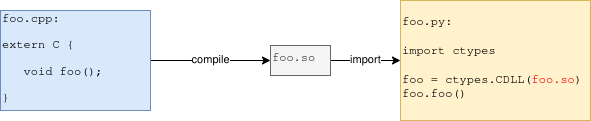
\includegraphics[width=\textwidth]{figures/Ctypes_schema.png}
    \caption{ctypes Schema}
    \label{fig:ctypes-schema}
\end{figure}



\subsubsection{Cython: Compiled Python Extensions}

Cython allows for the compilation of Python-like code into optimized C, potentially yielding performance improvements. It is suitable for creating C extensions and bridging Python with external C libraries. However, its effectiveness in wrapping existing C++ libraries may vary, as it may not fully leverage the library's pre-existing design. \cite{cython-docu}

\begin{figure}[htpb]
    \centering
    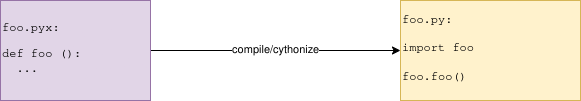
\includegraphics[width=\textwidth]{figures/cython_schema.png}
    \caption{Cython Schema}
    \label{fig:cython-schema}
\end{figure}

\subsubsection{pybind11: Modern C++ Bindings}

pybind11 is a header-only library designed to simplify the creation of Python bindings for C++ code. It leverages compile-time introspection to minimize boilerplate and offers robust support for modern C++ features, including templates and \ac{STL} data structures. Its design prioritizes ease of use and maintainability. \cite {pybind11-docu}

\begin{figure}[htpb]
    \centering
    \includegraphics[width=\textwidth]{figures/pybind_schema.png}
    \caption{pybind11 Schema}
    \label{fig:pybind11-schema}
\end{figure}

\subsubsection{Py-C-API: Native Python Extensions}

The Python/C API provides a direct mechanism for extending the Python interpreter with C or C++ modules. While offering high performance, it demands meticulous memory management and can result in less readable code. It is generally better suited for creating custom extensions than for wrapping existing libraries. \cite{py-c-api}

\begin{figure}[htpb]
    \centering
    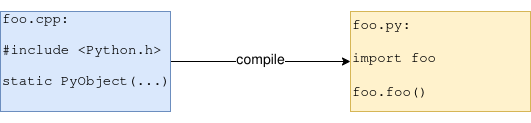
\includegraphics[width=\textwidth]{figures/python-C-API_schema.png}
    \caption{Python-C-API Schema}
    \label{fig:py-c-api-schema}
\end{figure}

\subsubsection{SWIG: Multi-Language Interface Generation}

SWIG is a tool capable of generating bindings for numerous programming languages. While it supports a broad range of C++ features, it introduces its own interface definition language, which may present a learning curve. Additionally, the necessity for manual type mappings can increase development effort. \cite{swig-docu}

\begin{figure}[htpb]
    \centering
    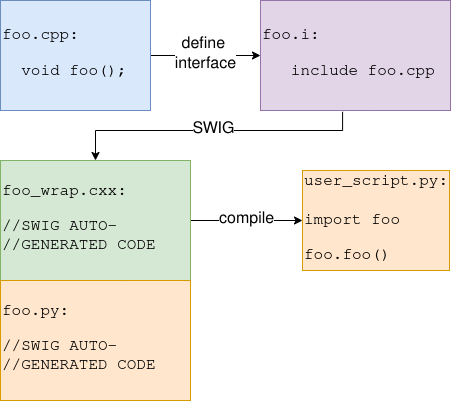
\includegraphics[scale=0.6]{figures/swig_schema.png}
    \caption{SWIG Schema}
    \label{fig:swig-schema}
\end{figure}


\subsubsection{Alternative Binding Tools}

Other tools, such as Boost.Python and Cffi, offer alternative approaches. Boost.Python, while powerful, introduces complex installation process. Cffi, primarily designed for C, may not fully support the complexities of modern C++ libraries, particularly those utilizing modern C++ features. \cite{boost-docu} \cite{cffi-docu}

As we can see there are plenty of technologies to integrate C++ in Python, using different approaches. Checking the performance of these tools is our next step to narrow down our choice.

\subsection{Performance Comparison}

Performance is a critical consideration, especially for tasks involving searching and updating components in large topologies. The overhead associated with each technology, including function calls and type casting, must be evaluated. In the following benchmarks we repeat the task a million times and measure the time it takes.

Initial tests involving file I/O operations indicate that Py-C-API offers the best performance, followed by pybind11 and SWIG. Python and Cython exhibit significantly lower performance due to the interpreter overhead.


\begin{figure}[htpb]
    \centering
  
    \pgfplotstableset{col sep=&, row sep=\\}
    
    % Define data for each method
    \pgfplotstableread{
      X & python & SWIG & PyBind11 & Py-C-API & Cython & ctypes \\
      5000  & 0.0676  & 0.0267  & 0.0302  & 0.0225  & 0.0767  & 0.0332  \\
      10000 & 0.1341  & 0.0504  & 0.0520  & 0.0417  & 0.1395  & 0.0622  \\
      15000 & 0.2017  & 0.0723  & 0.0775  & 0.0611  & 0.2075  & 0.0941  \\
      20000 & 0.2728  & 0.0966  & 0.1025  & 0.0796  & 0.2731  & 0.1286  \\
      25000 & 0.3446  & 0.1190  & 0.1256  & 0.0992  & 0.3430  & 0.1544  \\
      30000 & 0.4241  & 0.1458  & 0.1565  & 0.1216  & 0.4133  & 0.1843  \\
      35000 & 0.4883  & 0.1685  & 0.1817  & 0.1486  & 0.4849  & 0.2202  \\
      40000 & 0.5624  & 0.1960  & 0.2135  & 0.1642  & 0.5466  & 0.2375  \\
      45000 & 0.5938  & 0.2141  & 0.2261  & 0.1895  & 0.6389  & 0.2576  \\
      50000 & 0.6407  & 0.2365  & 0.2535  & 0.2029  & 0.7406  & 0.2919  \\
      55000 & 0.7169  & 0.2575  & 0.2797  & 0.2323  & 0.8013  & 0.3244  \\
      60000 & 0.7983  & 0.2930  & 0.2996  & 0.2533  & 0.8625  & 0.3440  \\
      65000 & 0.8724  & 0.3230  & 0.3209  & 0.2836  & 0.8962  & 0.3978  \\
      70000 & 0.9486  & 0.3455  & 0.3389  & 0.2902  & 0.9688  & 0.4048  \\
    }\datatable
  
    % Generate plot
    \begin{tikzpicture}
      \begin{axis}[
          ymin=0,
          legend style={legend pos=north west},
          grid=both,
          thick,
          ylabel={Execution Time (s)},
          xlabel={Probe Size},
          cycle list name=color list
        ]
  
        \addplot table[x=X, y=python]{\datatable}; 
        \addlegendentry{Python}
  
        \addplot table[x=X, y=SWIG]{\datatable}; 
        \addlegendentry{SWIG}
  
        \addplot table[x=X, y=PyBind11]{\datatable}; 
        \addlegendentry{PyBind11}
  
        \addplot table[x=X, y=Py-C-API]{\datatable}; 
        \addlegendentry{Py-C-API}
  
        \addplot table[x=X, y=Cython]{\datatable}; 
        \addlegendentry{Cython}
  
        \addplot table[x=X, y=ctypes]{\datatable}; 
        \addlegendentry{ctypes}
  
      \end{axis}
    \end{tikzpicture}
  
    \caption[Performance Comparison]{Execution time comparison for different Python interoperability methods.}
    \label{fig:performance-comparison}
  
    
  \end{figure}

The Python-C-API might be the optimal solution regarding performance, however, the documentation advises to better use a third party tool to simplify the process. \cite{py-c-api}

Therefore we only compare the performance of pybind11 and SWIG. To do this we create a datastructure that mimics sys-sage's internal representation in a very basic way. We then measure the time to get an object from a hierarchy of objects. 



\begin{figure}[htpb]
    \centering
  
    \pgfplotstableset{col sep=&, row sep=\\}
    \pgfplotstableread{
      x & swig & pybind11 \\
      10 & 2.267133142 & 7.590942619 \\
      20 & 4.028701226 & 9.500699417 \\
      30 & 5.918228375 & 12.46849245 \\
      40 & 7.794193961 & 12.67397027 \\
      50 & 9.38952239 & 14.04027122 \\
      60 & 10.9900335 & 14.36808235 \\
      70 & 13.0015907 & 16.24173763 \\
      80 & 14.8930638 & 17.69231723 \\
      90 & 16.45429449 & 18.234792 \\
      100 & 18.29529441 & 19.68409621 \\
      110 & 20.09700345 & 21.07857665 \\
      120 & 22.937185 & 22.91100467 \\
      130 & 23.55086321 & 25.18782614 \\
      140 & 25.76868722 & 26.28316 \\
      150 & 25.75257142 & 29.60488148 \\
      160 & 28.23660628 & 30.60642546 \\
      170 & 30.36670391 & 31.54023992 \\
      180 & 33.85480826 & 32.68026276 \\
      190 & 35.46123947 & 34.21423193 \\
      200 & 36.94181766 & 36.83799764 \\
      210 & 39.41546733 & 44.78271394 \\
      220 & 40.2630962 & 46.0669647 \\
      230 & 41.26109362 & 39.30260544 \\
      240 & 43.66919715 & 41.65095442 \\
      250 & 41.10896678 & 42.79613042 \\
      260 & 41.65160062 & 49.4102238 \\
      270 & 42.56338078 & 45.58386786 \\
      280 & 42.44157943 & 46.2824686 \\
      290 & 44.26966798 & 47.95827931 \\
      300 & 44.68688756 & 48.68347919 \\
    }\datatable
    \begin{tikzpicture}
      \begin{axis}[
          ymin=0,
          legend style={legend pos=north west},
          grid,
          thick,
          ylabel=Time (seconds),
          xlabel=Input Size
        ]
        \addplot+[mark=none]table[x=x, y=swig]{\datatable};
        \addlegendentry{SWIG}
        \addplot table[x=x, y=pybind11]{\datatable};
        \addlegendentry{PyBind11}
      \end{axis}
    \end{tikzpicture}
  
    \caption[Performance Comparison of SWIG and PyBind11]{Comparison of execution time between SWIG and PyBind11.}
    \label{fig:performance-swig-pybind11}
  \end{figure}
  

\begin{figure}[htpb]
    \centering
  
    \pgfplotstableset{col sep=&, row sep=\\}
    \pgfplotstableread{
      x & swig & pybind11 \\
      10 & 0.728748096 & 1.086200184 \\
      20 & 0.953306493 & 1.376843971 \\
      30 & 1.226998182 & 1.614387847 \\
      40 & 1.476429911 & 1.901537211 \\
      50 & 1.643896114 & 2.186163105 \\
      60 & 1.845129029 & 2.528576994 \\
      70 & 2.194456808 & 2.916303161 \\
      80 & 2.437852026 & 3.209785582 \\
      90 & 2.657877172 & 3.507811585 \\
      100 & 3.026818026 & 3.860601905 \\
      110 & 3.295786867 & 4.365836154 \\
      120 & 3.522095331 & 4.756411794 \\
      130 & 3.819491076 & 5.242209152 \\
      140 & 3.992675185 & 5.127110396 \\
      150 & 4.24713372 & 5.159396592 \\
      160 & 4.502797815 & 5.441533506 \\
      170 & 4.659608237 & 5.922976352 \\
      180 & 5.08548237 & 6.057849024 \\
      190 & 5.464223422 & 6.209325153 \\
      200 & 5.698968486 & 6.774561073 \\
      210 & 5.718441907 & 6.832615858 \\
      220 & 5.824529861 & 7.060233693 \\
      230 & 6.022517721 & 7.564672171 \\
      240 & 6.229809141 & 7.889981094 \\
      250 & 6.762351023 & 8.096503014 \\
      260 & 6.817011082 & 8.463510027 \\
      270 & 7.102505115 & 9.035682028 \\
      280 & 7.160332934 & 9.754081024 \\
      290 & 7.637865566 & 10.32763821 \\
      300 & 7.843654141 & 9.657189532 \\
    }\data
  
    \begin{tikzpicture}
      \begin{axis}[
          ymin=0,
          legend style={legend pos=north west},
          grid,
          thick,
          ylabel=Time (seconds),
          xlabel=Input Size
        ]
        \addplot+[mark=none] table[x=x, y=swig]{\data};
        \addlegendentry{SWIG -O3}
        \addplot+[mark=none] table[x=x, y=pybind11]{\data};
        \addlegendentry{PyBind11 -O3, reference option}
      \end{axis}
    \end{tikzpicture}
    \caption[Plot of SWIG and PyBind11]{A plot comparing the performance of SWIG and PyBind11 with optimization flag -O3.}\label{fig:swig-pybind11-plot}
  \end{figure}
\begin{figure}[hptb]
    \centering
  
    \pgfplotstableset{col sep=&, row sep=\\}
    \pgfplotstableread{
      x & swig & pybind11 \\
      10 & 0.831514591 & 1.058577497 \\
      20 & 1.127118936 & 1.471500208 \\
      30 & 1.4772158 & 1.761273233 \\
      40 & 1.736514494 & 2.126912437 \\
      50 & 2.025210358 & 2.46362231 \\
      60 & 2.214553424 & 2.804167879 \\
      70 & 2.603474917 & 3.326882148 \\
      80 & 2.877264073 & 3.673826322 \\
      90 & 3.352056939 & 3.967651672 \\
      100 & 3.392421572 & 4.391185498 \\
      110 & 3.703171002 & 4.916812021 \\
      120 & 4.275075549 & 5.214867283 \\
      130 & 5.214835618 & 5.347268902 \\
      140 & 6.241614607 & 5.945904962 \\
      150 & 6.595369415 & 6.519765277 \\
      160 & 6.967670258 & 7.11302645 \\
      170 & 7.165744065 & 7.452702384 \\
      180 & 7.80374477 & 7.193507064 \\
      190 & 8.358989104 & 7.662745811 \\
      200 & 8.92708868 & 7.899299085 \\
      210 & 9.175657786 & 8.070269308 \\
      220 & 9.27380257 & 8.513974392 \\
      230 & 9.771330559 & 8.768865073 \\
      240 & 10.07812149 & 8.980851734 \\
      250 & 10.57007511 & 9.686946998 \\
      260 & 10.93630689 & 9.962699361 \\
      270 & 11.02586082 & 10.96497769 \\
      280 & 11.80790557 & 10.70239503 \\
      290 & 12.17019807 & 11.02871699 \\
      300 & 12.6979764 & 11.43657468 \\
    }\data
  
    \begin{tikzpicture}
      \begin{axis}[
          ymin=0,
          ymax=20,
          legend style={legend pos=north west},
          grid,
          thick,
          ylabel=Time (seconds),
          xlabel=Hierarchy depth
        ]
        \addplot+[mark=none] table[x=x, y=swig]{\data};
        \addlegendentry{SWIG -O3, shared-pointers}
        \addplot+[mark=none] table[x=x, y=pybind11]{\data};
        \addlegendentry{PyBind11 -O3, shared-pointers}
      \end{axis}
    \end{tikzpicture}
    \caption[Plot of SWIG and PyBind11 with shared-pointers]{A plot comparing the performance of SWIG and PyBind11 with optimization flag -O3 and shared-pointers.}\label{fig:swig-pybind11-shared-pointers-plot}
  \end{figure}

The results show that SWIG is generally faster, except when using smart pointers. However, with our defined requirements, that not only involve performance we decide to go with pybind11.


\subsection{Technology Decision: pybind11 for Optimal Integration}

The selection of pybind11 as the primary technology for creating Python bindings for the sys-sage library stems from a comprehensive evaluation of various options, balancing performance, maintainability, and ease of use. While performance benchmarks indicated that SWIG might offer a slight speed advantage in certain scenarios, particularly with standard data structures, the crucial consideration of developer experience and long-term maintainability tipped the scales in favor of pybind11.

A significant drawback of SWIG is its reliance on a unique interface definition language. This necessitates that developers learn a new syntax, distinct from both C++ and Python, which can impede development speed and increase the learning curve for new contributors. In contrast, pybind11, being a header-only library embedded within C++, offers a more intuitive and familiar development environment for C++ programmers. This direct integration with C++ simplifies the process of creating and maintaining bindings, making it easier for future developers to understand and extend the project.

This decision aligns with findings from independent benchmarks, such as those presented in the \autoref{chapter:Related Work}, which highlight pybind11's superior usability despite potential performance trade-offs. The ease of integration and the reduced cognitive load for developers translate to faster development cycles and improved maintainability—critical factors for the long-term success of the sys-sage library's Python interface.

Furthermore, pybind11's robust support for C++ features, including \ac{STL} containers and inheritance, aligns perfectly with the sys-sage library's complexity. Its ability to seamlessly handle these features simplifies the wrapping process and ensures that the Python interface accurately reflects the C++ library's functionality. This comprehensive feature support, combined with its ease of use, makes pybind11 the optimal choice for creating a maintainable and extensible Python interface for the sys-sage library.
\chapter{Implementation}\label{chapter:Implementation}

\section{Project Structure}

The Python bindings for the sys\_sage library are encapsulated within a dedicated wrapper file. This file serves as the primary interface between the C++ library and the Python environment, ensuring a structured and maintainable codebase. The general layout of this file is as follows:
\begin{figure}[htpb]
    \centering
    \begin{tabular}{c}
        \begin{lstlisting}[language=C++]
            #include <pybind11/pybind11.h>
            #include <pybind11/stl.h>
            #include <pybind11/attr.h>
            #include "sys-sage.hpp"
            
            // Global variables and helper functions
            
            PYBIND11_MODULE(sys_sage, m) {
                // Expose C++ Macros to Python
                m.attr("COMPONENT_NONE") = SYS_SAGE_COMPONENT_NONE;
            
                // Bind the Component class
                py::class_<...>(m, "Component", ..., "Generic Component")
                    // Bind the constructor(s)
                    .def(py::init<...>())
                    // Bind member functions
                    .def("InsertChild", &Component::InsertChild, ...)
                    // Bind properties (getters and setters)
                    .def_property("parent", &Component::GetParent, &Component::SetParent, ...);
            
                // Bind module-level functions
                m.def("parseCccbenchOutput", &parseCccbenchOutput, ...);
            }
            \end{lstlisting}
    \end{tabular}
    \caption[Structure of the wrapper file]{The structure of the wrapper file.}\label{fig:wrapper-structure}
  \end{figure}


This structure is designed to provide a clear and organized layout, facilitating easy navigation and modification of the bindings. The file is segmented into distinct sections, each serving a specific purpose:

\begin{itemize}
    \item   \textbf{Include Directives:} Essential header files, including those from pybind11 and the sys\_sage library, are included to provide the necessary functionalities.
    \item   \textbf{Global Variables and Helper Functions:} This section accommodates any global variables or helper functions required for the bindings.
    \item   \textbf{PYBIND11\_MODULE Macro:} This macro defines the Python module and its contents. Within this macro, the following elements are defined:
        \begin{itemize}
            %TODO This is not really true
            \item   \textbf{DATA:} C++ macros are exposed to Python in form of module attributes, allowing Python code to use these as constants.
            \item   \textbf{Class Bindings:} C++ classes are bound to Python classes using \verb|py::class_<>|. This includes defining constructors, methods, and properties.
            \item   \textbf{Module Functions:} C++ functions that are not class methods are bound to the Python module itself.
        \end{itemize}
\end{itemize}

This structured approach ensures that the bindings are well-organized and easy to maintain, providing a solid foundation for the Python interface of the sys\_sage library.


\section{Object-Oriented Programming with pybind11}

\subsection{Class Definitions}

Python and C++ both offer object-oriented programming. C++ differentiates between structs and classes, while Python primarily uses classes. pybind11 allows C++ structs as well as classes to be bound to act like Python classes.

For each functionality, a table is provided for comparison.
        
\begin{table}[htbp]
\centering
\begin{tabular}{|l|l|}
\hline
\textbf{C++ implementation} &
\begin{lstlisting}[language=C++]
class Component {
    // ...
};
\end{lstlisting}
\\ \hline
\textbf{Pybind11-Binding} &
\begin{lstlisting}[language=C++]
py::class_<Component, std::unique_ptr<Component, py::nodelete>>(
    m, "Component", "Generic Component"
);
\end{lstlisting}
\\ \hline
\textbf{C++ usage} &
\verb|Component;| \\ \hline
\textbf{Python usage} &
\verb|sys_sage.Component| \\ \hline
\end{tabular}
\caption{Class Definition Comparison}
\label{tab:class_definition}
\end{table}

Header files define classes. pybind bindings are defined in the binding file within the module. To use \verb|sys-sage| in C++, we need to include \verb|syssage.hpp| in the project. To use \verb|sys-sage| in Python, we need to include \verb|sys_sage|, where we can also rename the module.

We can see that pybind bindings are straightforward. We use \verb|py::class_<T>| where \verb|T| is the template input, in this case, \verb|Component|. As mentioned in the previous chapter, for pybind to indicate that component objects should not be destroyed by Python, we use \verb|std::unique_ptr<T>| as holder type for the Component class, and we add a delete function, that is \verb|py::nodelete|. There are also other methods to define how Python should handle the underlying C++ objects.

The \verb|py::class_| takes the module, class name , and class documentation as arguments.

%*TODO:* Improve Documentation. Helpful feature to add documentation to the project and help users understand usage better.

\subsection{Constructor}

If we would define a class in native Python, it might look like this:

\begin{lstlisting}[language=Python, xleftmargin=4em, frame = single]
class Example(self):
    def __init__(self, id, name):
        self.id = id
        self.name = name
\end{lstlisting}

With pybind, we can take already defined Constructors of C++ implementation and can use the convenience function \verb|init<>()| that binds automatically the C++ Constructors.

\begin{table}[htbp]
\centering
\begin{tabular}{|l|l|}
\hline
\textbf{C++ implementation} &
\begin{lstlisting}[language=C++]
Component(
    int id = 0,
    string name = "unknown",
    int componentType = SYS_SAGE_COMPONENT_NONE
);
\end{lstlisting}
\\ \hline
\textbf{Pybind11-Binding} &
\begin{lstlisting}[language=C++]
.def(
    py::init<int, string, int>(),
    py::arg("id") = 0,
    py::arg("name") = "unknown",
    py::arg("type") = SYS_SAGE_COMPONENT_NONE
)
\end{lstlisting}
\\ \hline
\textbf{C++ usage} &
\verb|new Component();| \\ \hline
\textbf{Python usage} &
\verb|sys_sage.Component()| \\ \hline
\end{tabular}
\caption{Constructor Comparison}
\label{tab:constructor}
\end{table}

C++ implementation provides a bunch of Constructors for Component-Class and Subclasses. In our use case, Pybind's convenience function is indeed convenient.

For all functions and properties we want to bind to, we use \verb|.def(...)|. That also applies to initialization function, where we use the function \verb|py::init<T>()|. As one can see, this is a template function, and we replace \verb|T| with all the types of the Arguments there are defined in the C++ Constructor. In our example case, we have \verb|int|, \verb|string|, \verb|int| in this order.

As in every definition of a function in the bindings, we can use \verb|py::arg| to not only define default values but also we can give the argument names for the documentation. In this case, this might look like this: \verb|py::arg("id") = 0|. Instead of this, there is also a shorthand notation that would look like this: \verb|"id"_a=0|. However, the literal operator must be made visible before with \verb|using namespace pybind11::literals|.
\begin{lstlisting}[language=C++, xleftmargin=4em, frame = single]
            // Component-constructor without parent
            .def(
                py::init<int, string, int>(),
                py::arg("id") = 0,
                py::arg("name") = "unknown",
                py::arg("type") = SYS_SAGE_COMPONENT_NONE
            )
            
            // Component-constructor with parent
            .def(
                py::init<Component *, int, string, int>(),
                py::arg("parent"),
                py::arg("id") = 0,
                py::arg("name") = "unknown",
                py::arg("type") = SYS_SAGE_COMPONENT_NONE
            )
\end{lstlisting}
% *TODO:* Add shorthand notation in pybinds.
\subsection{Inheritance}

If we had to define Inheritance in Python, we can do it like this:
\newpage
\begin{lstlisting}[language=Python, xleftmargin=4em, frame = single]
class Vehicle:
    def honk(self):
        print("Honk!")

class Car(Vehicle):
    def drive(self):
        print("Vroom!")

my_car = Car()
my_car.honk()
my_car.drive()
\end{lstlisting}

The \verb|sys_sage| library has \verb|Component| as a generic class and many Component-Types as Subclasses. Inheritance should work properly, and indeed Pybind supports that.

\begin{table}[htbp]
\centering
\begin{tabular}{|l|l|}
\hline
\textbf{C++ implementation} &
\begin{lstlisting}[language=C++]
class Topology : public Component {
    // ...
};
\end{lstlisting}
\\ \hline
\textbf{Pybind11-Binding} &
\begin{lstlisting}[language=C++]
py::class_<
    Topology,
    std::unique_ptr<Topology, py::nodelete>,
    Component
>(m, "Topology")
\end{lstlisting}
\\ \hline
\textbf{C++ usage e.g.} &
\begin{lstlisting}[language=C++]
t.GetId();  // t is Topology, but can access Component's 
            // attributes and functions
\end{lstlisting}
\\ \hline
\textbf{Python usage} &
\verb|t.id # Works as in C++| \\ \hline
\end{tabular}
\caption{Inheritance Comparison}
\label{tab:inheritance}
\end{table}

The super-class is given as input in the template of \verb|py::class_<>|. Pybind will automatically care that all the functions and attributes from the super class are accessible to the Subclass. Multiple inheritance is also allowed. This is not yet needed but maybe in the future.

\subsection{Functions}

With pybind, binding functions is quite simple. Consider this C++ function for example:

\begin{table}[htbp]
\centering
\begin{tabular}{|l|l|}
\hline
\textbf{C++ implementation} &
\begin{lstlisting}[language=C++]
void Component::InsertChild(Component * child){
    // ...
}
\end{lstlisting}
\\ \hline
\textbf{Pybind11-Binding} &
\begin{lstlisting}[language=C++]
.def(
    "InsertChild",
    &Component::InsertChild,
    py::arg("child")
)
\end{lstlisting}
\\ \hline
\textbf{C++ usage e.g.} &
\verb|c->InsertChild(child);| \\ \hline
\textbf{Python usage} &
\verb|c.InsertChild(child)| \\ \hline
\end{tabular}
\caption{Function Comparison}
\label{tab:function}
\end{table}

In \verb|.def()|, the first argument is the name of the method. Normally in Python, the convention is to use snake-case for the method-name. In this case, we use the same name as in the C++ implementation. For some other specific methods, we use more simple names, but more on this in the “Attribute”-Section. The next argument is the C++ function to bind, and the last argument is the argument name for the function. This is not necessary, but it helps for documentation and allows usage of keyword arguments.

\subsection{Overloaded methods}

To use overloaded methods, we need to pick up the method signature to map the correct overloaded method.
\newpage
\begin{table}[htbp]
\centering
\begin{tabular}{|l|l|}
\hline
\textbf{C++ implementation} &
\begin{lstlisting}[language=C++]
void Component::PrintSubtree() {
    PrintSubtree(0);
}

void Component::PrintSubtree(int level) {
    PrintSubtree(0);
}
\end{lstlisting}
\\ \hline
\textbf{Pybind11-Binding} &
\begin{lstlisting}[language=C++]
.def(
    "PrintSubtree",
    (void (Component::)()) &Component::PrintSubtree,
    "Print the subtree of the component"
)

.def(
    "PrintSubtree",
    (void (Component::)(int)) &Component::PrintSubtree,
    "Print the subtree ..."
)
\end{lstlisting}
\\ \hline
\textbf{C++ usage e.g.} &
\begin{lstlisting}[language=C++]
c.PrintSubtree();
c.PrintSubtree(0);
\end{lstlisting}
\\ \hline
\textbf{Python usage} &
\begin{lstlisting}[language=Python]
c.PrintSubtree()
c.PrintSubtree(0)
\end{lstlisting}
\\ \hline
\end{tabular}
\caption{Overloaded Methods Comparison}
\label{tab:overloaded_methods}
\end{table}

The only difference to “normal” binding is that with overloading, we add the method signature, which is in this case \verb|void (Component::) ()| and \verb|void (Component::) (int)| respectively, which we add before \verb|&Component::PrintSubtree|.

%*TODO:* Maybe add more?

\subsection{Lambda functions}

In some cases, we don't have any C++ function we can bind to. This is because either we want to add some additional methods or there is some logic needed before the C++ function can be called.

For the first case, we have this example:
\newpage
\begin{lstlisting}[language=C++, xleftmargin=4em, frame = single]
.def(
    "__bool__",
    [](Component\& self){
        std::vector<Component*> children = self.GetChildren();
        return !children->empty();
    }
)
\end{lstlisting}

Here, we define the bool-function, which is called whenever we want to extract a bool value from an object of any type, in this case Component-type. Within the lambda function, we check if the Component object has any children. This is convenient because we can then in Python do this:

\begin{lstlisting}[language=Python,xleftmargin=4em, frame = single]
comp = sys_sage.Component()
# ...
if comp:
    # comp has children
else:
    # comp has no children
\end{lstlisting}

So this is an example for an extra feature that is not there in the base implementation of \verb|sys_sage| in C++. But this also shows that there it is quite straightforward to add more functionalities with a few lines of code.

\subsection{Module functions}

Previously presented methods are class methods, but there are also module functions that are not to be accessed over an object but see for yourself:

\begin{table}[htbp]
\centering
\begin{tabular}{|l|l|}
\hline
\textbf{C++ implementation} &
\begin{lstlisting}[language=C++]
int parseCapsNumaBenchmark(
    Component* rootComponent,
    string benchmarkPath,
    string delim
){
    // ...
}
\end{lstlisting}
\\ \hline
\textbf{Pybind11-Binding} &
\begin{lstlisting}[language=C++]
m.def(
    "parseCapsNumaBenchmark",
    \&parseCapsNumaBenchmark,
    py::arg("root"),
    py::arg("benchmarkPath"),
    py::arg("delim") = ";"
);
\end{lstlisting}
\\ \hline
\textbf{C++ usage e.g.} &
\verb|parseCapsNumaBenchmark( root, “benchmark.csv”, “;”);| \\ \hline
\textbf{Python usage} &
\verb|sys_sage.parseCapsNumaBenchmark(root, "benchmark.csv", ";")| \\ \hline
\end{tabular}
\caption{Module Function Comparison}
\label{tab:module_functions}
\end{table}

So this is quite similar to the class methods, but here we assign the function to the module interface object \verb|m|.
\newpage


\section{Attributes}

This section delves into the intricacies of attributes within the \verb|sys_sage| library, expanding on the object-oriented programming concepts discussed earlier. Attributes warrant a dedicated discussion due to the numerous special cases and module-specific considerations.

\subsection{Module Attributes}

\verb|sys_sage| employs macros in its C++ implementation to define component and datapath types. To maintain consistency and offer similar functionality in Python, we utilize module attributes. 

\begin{table}[htbp]
\centering
\begin{tabular}{|l|l|}
\hline
\textbf{C++ implementation} & \begin{lstlisting}[language=C++]
#define SYS_SAGE_COMPONENT_NONE 1 
\end{lstlisting} \\ \hline
\textbf{Pybind11-Binding} & \begin{lstlisting}[language=C++]
m.attr("COMPONENT_NONE") = SYS_SAGE_COMPONENT_NONE;
\end{lstlisting} \\ \hline
\textbf{C++ usage e.g.} & \verb|c.CountAllSubcomponentsByType(SYS_SAGE_COMPONENT_NONE);| \\ \hline
\textbf{Python usage} & \verb|c.CountAllSubcomponentsByType(sys_sage.COMPONENT_NONE)| \\ \hline
\end{tabular}
\caption{Module Attribute Comparison}
\label{tab:module_attributes}
\end{table}

In C++, these macros are preprocessed and replaced with their corresponding integer values. In Python, they are treated as exported variables, registered using the \verb|attr| function, effectively making them module attributes. Pybind handles the necessary type casting, as all macros resolve to integers.

A naming convention is employed where the “SYS\_SAGE” prefix is omitted from the Python attribute names to avoid redundancy. As demonstrated in the example, the attributes are accessed via \verb|sys_sage.COMPONENT_NONE|.
%TODO Add acronym
A significant advantage of the Python implementation is its enhanced documentation capabilities. A user's \ac{IDE} or the \verb|help(sys_sage)| function in python can display all module attributes within the DATA section, aiding users in selecting the appropriate options.

\subsection{Properties (Default Attributes)}

In C++, class attributes are typically private and accessed through setter and getter methods. However, this pattern is not idiomatic in Python. Pybind offers the \verb|def_property| function to bind setter and getter methods to Python properties, providing a more natural syntax.

\begin{table}[htbp]
\centering
\begin{tabular}{|l|l|}
\hline
\textbf{C++ implementation} & \begin{lstlisting}[language=C++]
class Component{
  private:
     string name;
};
...
void SetName(string name){...}
string GetName(){...}
\end{lstlisting} \\ \hline
\textbf{Pybind11-Binding} & \begin{lstlisting}[language=C++]
.def_property("name", &Component::GetName, &Component::SetName)
\end{lstlisting} \\ \hline
\textbf{C++ usage e.g.} & \begin{lstlisting}[language=C++]
string name = c.GetName();
c.SetName("name");
\end{lstlisting} \\ \hline
\textbf{Python usage} & \begin{lstlisting}[language=Python]
name = c.name
c.name = "name"
\end{lstlisting} \\ \hline
\end{tabular}
\caption{Property Comparison}
\label{tab:properties}
\end{table}
\newpage
This syntax is more intuitive for Python users. Pybind also provides \verb|def_property_readonly| for read-only properties, such as the \verb|id| attribute.

\begin{table}[htbp]
\centering
\begin{tabular}{|l|l|}
\hline
\textbf{C++ implementation} & \begin{lstlisting}[language=C++]
class Component{
  private:
     int id;
};
...
string GetId(){...}
\end{lstlisting} \\ \hline
\textbf{Pybind11-Binding} & \begin{lstlisting}[language=C++]
.def_property_readonly("id", &Component::GetId)
\end{lstlisting} \\ \hline
\textbf{C++ usage e.g.} & \verb|int id = c.GetId();| \\ \hline
\textbf{Python usage} & \verb|id = c.id| \\ \hline
\end{tabular}
\caption{Read-only Property Comparison}
\label{tab:readonly_properties}
\end{table}

\subsection{Dynamic Attributes}

Python natively supports dynamic attributes, allowing users to add attributes to objects at runtime.

\begin{lstlisting}[language=Python, xleftmargin=4em, frame = single]
class Dog():
    # no attributes defined here
    ...

d = Dog()
d.hungry = True
d.hungry # True
\end{lstlisting}

This behavior is desirable for \verb|sys_sage| components and datapaths, especially considering the C++ implementation's \verb|std::map<std::string, void*> attrib| which facilitates dynamic attribute storage.

\subsubsection{Attribute-Map}

The \verb|attrib| map offers high flexibility and performance by storing \verb|void*| pointers with string keys. This allows for storing both C++ types for the default attributes and Python types for custom attributes. Users should be able to modify these attributes, mirroring the C++ base implementation.

There are multiple possibilities to connect the \verb|attrib| map to Python attributes. For example, Pybind can activate Python's native dynamic attribute functionality using \verb|py::dynamic_attr()|.

\begin{lstlisting}[language=C++, xleftmargin=4em, frame = single]
py::class_<Component, std::unique_ptr<Component, py::nodelete>>(m, "Component", py::dynamic_attr(),"Generic Component");
\end{lstlisting}

This enables dynamic attribute usage in Python:

\begin{lstlisting}[language=Python, xleftmargin=4em, frame = single]
c = sys_sage.Component()
c.dynamic = "attribute"
c.dynamic # returns "attribute"
\end{lstlisting}

However, this approach conflicts with \verb|def_property()|. If we want to conntect the \verb|attrib| map to Python attributes we need to override the \verb|__setattr__| and \verb|__getattr__| methods, but this breaks property functionality. Handling properties like \verb|name| or \verb|id| in custom setter and getter methods, that we define would work as well, but results in bloated code. Therefore, an alternative solution is considered. This approach uses the \verb|[]| operator to access attributes, overriding \verb|__getitem__| and \verb|__setitem__|.

\begin{lstlisting}[language=Python, xleftmargin=4em, frame = single]
c = sys_sage.Component()
# solution with dynamic attributes
c.example = "test"      # calls __setattr__
c.example               # calls __getattr__
# solution with items
c["example"] = "test"   # calls __setitem__
c["example"]            # calls __getitem__
\end{lstlisting}

This solution avoids conflicts with other functions.

% The implementation in the bindings is as follows:

% \begin{lstlisting}[language=C++, xleftmargin=4em, frame = single]
% .def("__setitem__", [](Component& self, const std::string& name, py::object value) {
%     set_attribute(self,name, value);
% })
% .def("__getitem__", [](Component& self, const std::string& name) {return get_attribute(self,name);
% })
% .def("__getitem__", [](Component& self, int pos) {
%     return get_attribute(self,pos);
% })
% .def("__delitem__", [](Component& self, const std::string& name) {remove_attribute(self,name);
% })
% \end{lstlisting}

Overloaded \verb|__getitem__| methods allow access by key and index. The following example demonstrates this:

\begin{lstlisting}[language=Python, xleftmargin=4em, frame = single]
c["example"] = "test"
c[0]  # returns "test" if "example" is the only custom attribute
\end{lstlisting}
In the Python implementation, accessing and modifying attributes is designed to be user-friendly. The getter and setter methods for attributes are implemented to handle Python objects of any type or default attributes. This abstraction allows users to interact with custom attributes without explicit type casting. For default attributes, users need to be aware of the corresponding Python types.

In contrast, the C++ implementation requires more explicit memory management and type handling for attribute manipulation. The following code snippet illustrates the process of updating and retrieving an attribute in C++:

\begin{lstlisting}[language=C++, xleftmargin=4em, frame = single]
// Update Attribute
std::string key = "example";
if (c->attrib.find(key) != c->attrib.end()) {
    std::string* oldValue = static_cast<std::string*>(c->attrib[key]);
    delete oldValue; // Free the old value
}
std::string* newValue = new std::string("test"); // Allocate new value
c->attrib[key] = static_cast<void*>(newValue); // Update the map

// Retrieve Attribute
if (c->attrib.find(key) != c->attrib.end()) {
    std::string* retrievedValue = static_cast<std::string*>(c->attrib[key]);
    std::cout << "Value: " << *retrievedValue << std::endl;
} else {
    std::cout << "Key not found." << std::endl;
}
\end{lstlisting}

As demonstrated in the code, updating an attribute in C++ involves checking for the existence of the key, explicitly freeing the memory associated with the old value, allocating memory for the new value, and then updating the attribute map with a void pointer. Similarly, retrieving an attribute requires casting the void pointer back to the expected type after verifying the key's existence. This manual memory management and type casting in C++ contrasts with the more dynamic and implicit handling of attributes in the Python interface provided by Pybind11.
In the following we briefly explain the helper functions that are used:

The \verb|set_attribute| function examines default values, converts data to C++ types, encapsulates Python data types in shared pointers, and stores them in the \verb|attrib_map|. The \verb|get_attribute| function retrieves attributes using a key or an index and casts the \verb|void*| pointers to their appropriate types. The \verb|del_attribute| function removes attributes from the map.

For the Component class the second approach, using items, was chosen for its simplicity and compatibility with existing properties. For Datapaths however dynamic attributes were enabled. Since the \verb|attrib| map is not being used in the xml export and import functionality we use the native Python dynamic attributes there.

\section{XML Export}

\subsection{Original Implemented Functionality}

The base C++ implementation of \verb|sys_sage| includes XML export functionality, which traverses the topology and generates an XML representation of it. XML's hierarchical structure is well-suited for representing topologies, where the topology itself is the root node, cores and threads are leaf nodes, and various components reside in between.

XML properties are utilized to represent default attributes such as \verb|id|, \verb|name|, \verb|type|, and type-bound memory attributes like \verb|size|. Datapaths are also included, with attributes like \verb|src|, \verb|target|, \verb|orientation|, \verb|latency|, and \verb|bandwidth|.

Dynamic attributes, which users can add in C++, are represented as separate XML nodes:

\begin{lstlisting}[language=xml, xleftmargin=4em, frame = single]
<Attribute name="GPU_Clock_Rate">
    <GPU_Clock_Rate frequency="2.000000" unit="MHz"/>
</Attribute>
\end{lstlisting}

Since the \verb|attrib| map in C++ stores attributes as \verb|void*|, the XML export function requires user-defined functions to parse custom attribute types. Users can define up to two functions:

\begin{lstlisting}[language=C++, xleftmargin=4em, frame = single]
std::function<int(string,void*,string*)> search_custom_attrib_key_fcn;
std::function<int(string,void*,xmlNodePtr)> search_custom_complex_attrib_key_fcn;
\end{lstlisting}

The first function returns a string representation of the attribute, while the second allows for creating more complex XML nodes. The export function can be called as follows:

\begin{lstlisting}[language=C++, xleftmargin=4em, frame = single]
exportToXml(
    root, 
    path, 
    search_custom_attrib_key_fcn, 
    search_custom_complex_attrib_key_fcn
);
\end{lstlisting}

\subsection{Process Description}

The Python implementation of \verb|exportToXml| mirrors the C++ functionality, allowing users to define custom parsing functions as in this example:

\begin{lstlisting}[language=Python, xleftmargin=4em, frame = single]
def search_custom(key: str, value) -> str:
    if "example" in key:
        return str(value)+"test"
    return None

def search_custom_complex(key: str, value) -> str:
    return "<root><Attribute key=\"" + str(key) + "\" value=\"" + str(value) + "\"/><root>"
\end{lstlisting}

The \verb|key| is always a string, while \verb|value| can be any Python type. The return value must be a string, representing either a simple value or an XML node respectively. When creating the XML node string for complex attributes the target XML information is incapsulated in a tag that is ommitted in the parsing operation. XML parsing modules like \verb|xml.etree.ElementTree|\cite{xml-etree} can be used to construct complex XML nodes.

The Python export function can be called as follows:

\begin{lstlisting}[language=Python, xleftmargin=4em, frame = single]
sys_sage.exportToXml(root, "out.xml", search_custom, search_custom_complex)
\end{lstlisting}

% The Pybind bindings are defined as follows:

% \begin{lstlisting}[language=C++, xleftmargin=4em, frame = single]
% m.def("exportToXml", [](Component& root, string xmlPath, std::optional<py::function> print_att = std::nullopt, std::optional<py::function> print_catt = std::nullopt) {
%         if(print_att)
%             print_attributes = *print_att;
%         if(print_catt)
%             print_complex_attributes = *print_catt;
%         exportToXml(&root, xmlPath,print_att ? xmldumper : nullptr,print_catt ? xmldumper_complex : nullptr);
%     },py::arg("root"), py::arg("xmlPath") = "out.xml", py::arg("print_att") = py::none(), py::arg("print_catt") = py::none());
% \end{lstlisting}

Global variables are used to store the user-defined functions. Two helper functions are used to translate between Python and C++ types. The helper functions implement the required functions with the correct signature for the XML-export function and within the helper functions the user-defined Python functions - previously stored in the global variables - are called to achieve the desired functionality. Default attributes are skipped, but this can be changed in the future.

\subsection{Helper Functions}

In the following we explain which steps are performed by the helper functions:

\subsubsection{Simple Attributes}
\begin{enumerate}
\item Check if the attribute is a default attribute. If yes, skip it.
\item Cast the \verb|void*| to a Python object.
\item Call the user-defined Python function, passing the key and value (Python object).
\item Cast the returned Python string to a C++ string.
\item Store the string in the return string pointer.
\end{enumerate}

\subsubsection{Complex Attributes}
\begin{enumerate}
\item Follow steps 1-3 for simple attributes.
\item Expect user-defined function to return XML node as a Python string.
\item Convert Python string to C++ string.
\item Parse the XML node using \verb|xmlParseDoc| \cite{libxml2-docu} and add it to the XML node.
\end{enumerate}

% \begin{lstlisting}[language=C++, xleftmargin=4em, frame = single]
% xmlDocPtr doc = xmlParseDoc((const xmlChar*)xml_str.c_str());
% xmlNodePtr root = xmlDocGetRootElement(doc);
% xmlAddChild(node,root->children);
% \end{lstlisting}

\section{XML Import}

The XML import function mirrors the XML export function, operating in reverse. This section provides a detailed explanation of the import function's inner workings, as it represents a new feature in the C++ base implementation.

\subsection{Process Description}

The XML import process involves the following steps:

\begin{enumerate}
    \item \textbf{Read XML File:} The function begins by reading the input XML file.
    \item \textbf{Find Component and Datapath Nodes:} It then locates component and datapath nodes within the XML structure.
    \item \textbf{Traverse Components:} The function recursively traverses all components, adding them to a map of addresses (obtained from the XML file) and newly created component instances.
    \item \textbf{Attribute Collection:} Upon encountering an attribute node, the function calls an attribute collection routine. This routine attempts to parse attributes using the following order:
        \begin{enumerate}
            \item Custom function for simple attributes.
            \item Default function for simple attributes.
            \item Custom function for complex attributes.
            \item Default function for complex attributes.
        \end{enumerate}
        If no parsing method succeeds, the attribute is omitted.
    \item \textbf{Add Datapaths:} Datapaths are created by inspecting the component map, which stores components and their corresponding addresses from the XML file. This ensures correct connection of datapaths to the created components.
    \item \textbf{Return Root Component:} The function returns the root component, which is of type Topology.
\end{enumerate}

\subsection{User-Defined Functions}

Users can provide custom functions for attribute parsing:

    \begin{lstlisting}[language=C++, xleftmargin=4em, frame = single]
    std::function<void*(xmlNodePtr)> search_custom_attrib_key_fcn = NULL;
    \end{lstlisting}
    The function for simple attributes receives an \verb|xmlNodePtr| and returns a \verb|void*| to store the attribute value in the \verb|attrib| map.

    \begin{lstlisting}[language=C++, xleftmargin=4em, frame = single]
    std::function<int(xmlNodePtr, Component *)> search_custom_complex_attrib_key_fcn = NULL;
    \end{lstlisting}
    The function for complex attributes receives an \verb|xmlNodePtr| and a pointer to the current component. It allows users to configure component properties directly via the \verb|attrib| map. The function must return 1 for success and 0 for failure.

    Similar to the export function the import function can be called like this:

    \begin{lstlisting}[language=C++, xleftmargin=4em, frame = single]
    Component* importFromXml(
        path, 
        search_custom_attrib_key_fcn, 
        search_custom_complex_attrib_key_fcn
    );
    \end{lstlisting}

\subsection{Python Interface}

Users can provide up to two functions in Python. Here is an example of how this can be done:

\textbf{Simple Attributes:}
    \begin{lstlisting}[language=Python, xleftmargin=4em, frame = single]
    def search_custom(x : str):
        if "example" in x:
            y = x.split("value=\"")[-1]
            return y.rstrip("\"/>")
        else:
            return None
    \end{lstlisting}

\textbf{Complex Attributes:}
    \begin{lstlisting}[language=Python, xleftmargin=4em, frame = single]
    def search_custom_complex(x : str,c : Component) -> int:
        x = str(x)
        m = re.search(r'<my_core_info\s+temperature="(\d*\.\d*)" temp_unit="(\w*)" frequency="(\d*)" freq_unit="(\w*)"/>', x)
        if m:
            my_core_info = {}
            my_core_info["temperature"] = float(m.group(1))
            my_core_info["temp_unit"] = m.group(2)
            my_core_info["frequency"] = int(m.group(3))
            my_core_info["freq_unit"] = m.group(4)
            c["my_core_info"] = my_core_info
            return 1
        else:
            return 0
    \end{lstlisting}

The \verb|importFromXml()| function can be called as follows:

\begin{lstlisting}[language=Python, xleftmargin=4em, frame = single]
sys_sage.importFromXml("in.xml", search_custom, search_custom_complex)
\end{lstlisting}

% The corresponding Pybind bindings are:

% \begin{lstlisting}[language=C++, xleftmargin=4em, frame = single]
% m.def("importFromXml",[](string path, std::optional<py::function> search_custom_attrib_key_fcn = std::nullopt, std::optional<py::function> search_custom_complex_attrib_key_fcn = std::nullopt) {
%         if(search_custom_attrib_key_fcn)
%             read_attributes = *search_custom_attrib_key_fcn;
%         if(search_custom_complex_attrib_key_fcn)
%             read_complex_attributes = *search_custom_complex_attrib_key_fcn;
%         return importFromXml(path,search_custom_attrib_key_fcn ? xmlloader : nullptr, search_custom_complex_attrib_key_fcn ? xmlloader_complex : nullptr );
%     }, py::arg("path"), py::arg("search_custom_attrib_key_fcn") = py::none(), py::arg("search_custom_complex_attrib_key_fcn") = py::none());
% \end{lstlisting}

We've already seen this approach in the export function,  where some global variables store the user-defined Python functions. Helper functions facilitate type conversion between Python and C++. In the next section the exact steps followed in these helper functions are explained.

\subsection{Helper Functions}
\textbf{Simple attributes:}
    \begin{enumerate}
        \item Dump the XML node content to a string.
        \item Cast the string to a Python string.
        \item Call the user-defined Python function with the Python string.
        \item Store the returned Python object in the \verb|attrib| map.
    \end{enumerate}
    \textbf{Complex attributes:}
    \begin{enumerate}
        \item Perform the same 2 steps as for simple attributes.
        \item Pass the string and the current component to the Python function.
        \item The Python function returns a success status (1 or 0).
    \end{enumerate}

Same as in export functionality we need the helper functions to implement the required functions with the proper signature. It is safe to say, that the import functionality gives the user more power, as he can directly access the component. 

\begin{figure}[htpb]
    \centering
    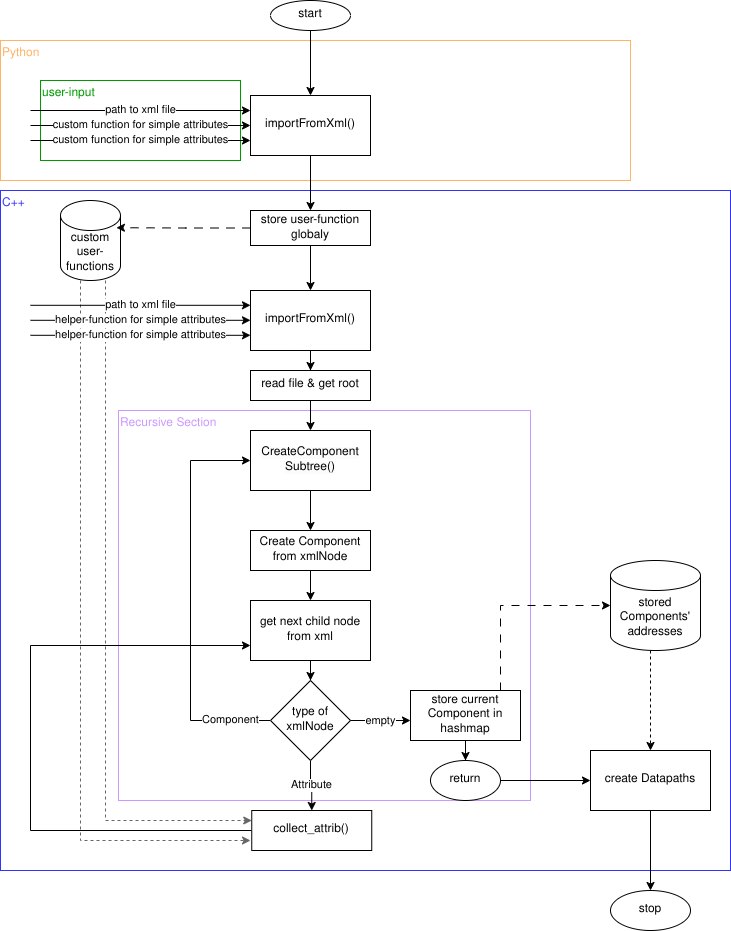
\includegraphics[width=\textwidth]{figures/XML_import-flowchart.png}
    \caption{XML Import Flowchart}
    \label{fig:xml-import}
\end{figure}

\begin{figure}[htpb]
    \centering
    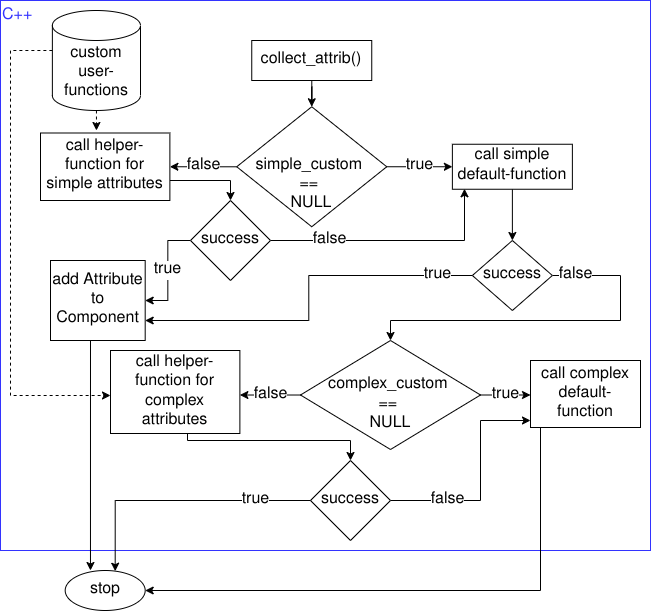
\includegraphics[width=\textwidth]{figures/Attribute_from_xml.png}
    \caption{Attribute parsing}
    \label{fig:Attribute parsing}
\end{figure}
\newpage
\section{Ownership Management and Return-Value Policies}

A critical challenge in interfacing C++ with Python involves the management of object ownership, particularly concerning the \verb|Component| objects within the sys\_sage library. By default, pybind11 transfers ownership of the underlying C++ object to the Python side. This implies that when a Python object, such as \verb|c = sys_sage.Component()|, is created, Python assumes responsibility for its lifecycle, including reference counting and deallocation. While this approach is generally adequate for objects without external dependencies, it becomes problematic when dealing with interconnected components, such as parent-child relationships or datapath associations.

Consider the following scenario:

  \begin{lstlisting}[language=Python, xleftmargin=4em, frame = single]
c = sys_sage.Component()
child = sys_sage.Component(c) # Parent set in constructor
del c
d = child.parent
print(d.id) # Undefined behaviour
  \end{lstlisting}

In this example, deleting \verb|c| in Python leads to the deallocation of the corresponding C++ object. However, the \verb|child| object retains a reference to the now-deleted parent. Consequently, accessing \verb|child.parent| results in undefined behavior, as the referenced object no longer exists. This issue arises because the \verb|Component| destructor does not update references in related objects, such as parent nodes, child nodes, or datapaths.

An initial attempt to address this problem involved implementing a custom delete function, \verb|delete(bool withSubtree)|, to replace the default destructor. However, this approach was deemed unsuitable due to potential conflicts with Python's garbage collection mechanism. As noted in pybind11's documentation, overriding the \verb|__del__(self)| method in Python is strongly discouraged, as it can interfere with the garbage collection process. \cite[see Chapter 12]{python-gc}

To mitigate these issues, pybind11's capability to disable ownership transfer was utilized. By modifying the template parameters of the \verb|py::class_<>| declaration, ownership of the C++ objects can be retained by the C++ side. Specifically, the \verb|std::unique_ptr<Component, py::nodelete>| template parameter was employed. The \verb|py::nodelete| keyword instructs pybind11 to prevent Python from deallocating the underlying C++ object. This ensures that the C++ side remains responsible for managing object lifetimes.

However, this solution introduces a new challenge. The base C++ program provides methods for manually deleting objects, which, when exposed to Python, can lead to inconsistencies. For instance:
\newpage
  \begin{lstlisting}[language=Python, xleftmargin=4em, frame = single]
import sys_sage

c = sys_sage.Component()
d = c
c.Delete()
d.Delete() #Segmentation Fault
  \end{lstlisting}
  

In this scenario, deleting \verb|c| using the \verb|Delete()| method deallocates the C++ object, but the Python wrapper \verb|d| remains unaware of this change. Ideally, all references to the deleted object should be updated. Unfortunately, pybind11 does not provide a mechanism for automatically updating these references. While this scenario is relatively rare, it underscores the need for careful consideration of object deletion strategies.

As mentioned before, pybind11, by default, invokes the destructor of the underlying C++ object when the reference count reaches zero. To enhance consistency, modifying the destructor to update relevant references is considered. 

\subsection{Destructor modifications}

In the base implementation, the destructors remain untouched. Consequently, to free resources, the user must explicitly call the \verb|Delete| function. This function provides the option to also delete the subtree, encompassing all descendants of the component. Naturally, all Datapaths connected to the component are deleted in this process. However, the attributes stored in the \verb|attrib| map are not automatically deallocated. Typically, in most containers from the \ac{STL}, memory is freed upon destruction for all contained items except pointers \cite{cppreference-map-destructor}.

As an alternative to the approach requiring explicit \verb|Delete| calls, thereby passing memory management to the C++ side, we now examine a solution utilizing custom destructors for the Component and Datapath classes. The following illustration, Figure \ref{fig:topo-example}, may help to grasp the details:
\begin{figure}[htpb]
    \centering
    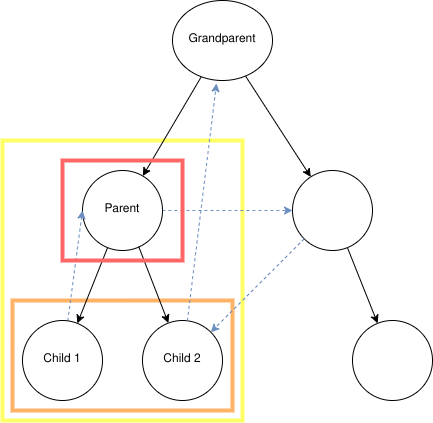
\includegraphics[scale=0.5]{figures/Topo-example.png}
    \caption{Topology Example}
    \label{fig:topo-example}
\end{figure}

To remove the "Parent" in this Topology, we no longer call the \verb|Delete| method. Instead, \verb|delete Parent| is used. In this solution, the Destructor removes all Datapaths connected to the Component. Additionally, Child 1 and 2, as well as the Grandparent, are updated: the children's \verb|parent| values are set to \texttt{NULL}, and Parent is removed from the Grandparent's children list. The children are no longer directly connected to their grandparent and can only be reached if a Datapath to another component remains. In our case, Child 1 becomes unreachable, as its only two connections — once in the Parent's children list and once via the Datapath to Parent — are destroyed with the deletion of Parent. This might also cause memory leaks if components fall out of scope without any remaining connection to the rest of the topology. Therefore, the user should always consider calling the \verb|DeleteSubtree| method beforehand, which has slight modifications compared to the base implementation but effectively achieves the same outcome.

The Datapath's destructor is also modified. Essentially, the logic behind the \verb|DeleteDatapath| method is migrated to the destructor.

The solution presented in this section is cleaner and allows for seamless usage of the pybind11 binding, enabling the Python interpreter to manage memory deallocation.
\chapter{Evaluation}\label{chapter:Evaluation}

The following evaluation chapter assesses the usability and performance of the developed Python interface for \texttt{sys-sage} against its C++ counterpart. It also examines the integration of the new XML import feature. Through benchmarks and qualitative analysis, we quantify the performance impact of the Python bindings and discuss the trade-offs between user-friendliness and efficiency. The evaluation mainly focuses on the Python implementation without the modifications to the destructors of the base implementation, therefore we discuss the strengths and weaknesses of the solution with the mentioned modifications.

\section{Requirement Analysis and Performance Evaluation}
First we want to revisit the requirements of the Python implementation of sys-sage, which are described in \autoref{chapter:Approach}, followed by a performance evaluation of the Python and C++ implementations.
\subsection{Library Complexity and Dependencies}

The Python solution mirrors the C++ implementation, encompassing nearly all functionalities. The only current limitation is the handling of overloaded methods, that accept a list of components as arguments. In that case the user must use the alternative method. 
\begin{lstlisting}[language=Python, xleftmargin=4em, frame = single]
    c.GetAllChildrenByType(children_list, type) # this won't work
    # do this instead 
    children_list += c.GetAllChildrenByType(type)
    \end{lstlisting}

Attributes can be stored as Python attributes, and both import and export functionalities are available, with optional support for custom Python functions to parse the attributes. One limitation is that currently the user has no control over default attributes when exporting to XML. 

The basic setup, excluding optional dependencies like \texttt{intel\_pqos} and \texttt{nvidia\_mig}, requires only two dependencies: Python and pybind11

\subsection{Error Handling and Documentation}

Simple error messages have been integrated, but there is room for improvement in error handling and user feedback. Basic documentation is provided, outlining the functionality of each function.

\subsection{Future Support and Build/Installation}

Pybind11 is a well-established tool for creating bindings, supported by an active community and ongoing maintenance. CMAKE support allows users to build either the Python or C++ version of sys-sage, providing flexibility in deployment.

\subsection{User Experience}

The Python interface offers a more user-friendly experience, enabling rapid prototyping and testing. For example, scheduling processes on HPC systems can be quickly prototyped and analyzed using Python scripts. If performance becomes a bottleneck, the solution can be transitioned to C++ for optimal execution. Memory management, however, requires careful attention, as users must manually manage subtree deletion to avoid undefined behavior. This work presents improvements to destructors, though memory management remains a complex aspect.

\subsection{Performance Benchmarking}

\subsubsection{Setup and Methodology}

To evaluate performance, C++ benchmarks utilize the high-resolution clock, while Python benchmarks employ the \texttt{timeit} module. The testing environment consisted of an Arch Linux system with an Intel i7-9750H CPU and 15GB of RAM.

It is important to acknowledge that precise benchmarking requires rigorous methodology, including accurate resource measurement, reliable process termination, deliberate core assignment, consideration of non-uniform memory access, avoidance of swapping, and isolation of individual runs. \cite{beyer2019reliable}

However, given the substantial performance disparities between Python and C++, the benchmarks presented herein provide a general overview. For use cases demanding high precision, adhering to established benchmarking standards is recommended.

The goal of this section is to compare the Python and C++ implementations to provide insights into the performance trade-offs associated with each language. As presented in the \autoref{chapter:Implementation} we have two different solutions for the Python implementation of sys-sage. For the evaluation we will only consider the solution without destructor modifications.

\subsubsection{Basic Functionality Performance}

\begin{center}
\begin{tabular}{lrrr}
\textbf{Function} & \textbf{Python (ns)} & \textbf{C++ (ns)} & \textbf{Factor} \\
\hline
Parsing HWloc & 2880354 & 1240570 & 2.32 \\
Parsing capsnuma & 4881208 & 365801 & 13.34 \\
Parsing mt4g & 71169350 & 52992073 & 1.34 \\
Getting HWloc subtree nodelist & 453509 & 14055 & 32.27 \\
Getting mt4g subtree nodelist & 26648203 & 589624 & 45.20 \\
Getting all components & 39845198 & 470893 & 84.62 \\
Getting numa max bw & 30936 & 70 & 441.94 \\
Creating new component & 17054 & 364 & 46.85 \\
\end{tabular}
\end{center}

The results indicate that parsing functions exhibit comparable performance. However, get operations, particularly retrieving all components, are significantly slower in Python due to the overhead of converting \texttt{std::vector} to Python lists. Creating new components is also considerably more expensive in Python, attributed to the inherent overhead of wrapping C++ objects for Python. The benchmarks to get the datapath with the max bandwidth from a component, which involves additional logic beyond a simple API call, demonstrates a substantial performance difference, highlighting the cost of loops in Python.

\subsubsection{XML Import and Export Performance}

\begin{center}
\begin{tabular}{lrrr}
\textbf{Function} & \textbf{Python (ns)} & \textbf{C++ (ns)} & \textbf{Factor} \\
\hline
\textbf{XML Import} & & & \\
Both functions & 1859323 & 387664 & 4.80 \\
Only simple & 175492 & 39347 & 4.46 \\
Only complex & 251298 & 35731 & 7.03 \\
None & 94179 & 37559 & 2.51 \\
\textbf{XML Export} & & & \\
Both functions & 209590 & 53481 & 3.92 \\
Only simple & 175346 & 50376 & 3.48 \\
Only complex & 225953 & 50914 & 4.44 \\
None & 163335 & 51095 & 3.20 \\
\end{tabular}
\end{center}

The XML import and export benchmarks, conducted with two components, where one of them has two attributes (one simple, one complex), reveal that the Python implementation with only complex attribute user functions is more costly. The C++ implementation, which directly writes to \texttt{xmlNodePtr}, is faster than the Python counterpart, which involves string conversions and parsing.

\subsubsection{Attribute Access Performance}

\begin{center}
\begin{tabular}{lrrr}
\textbf{Operation} & \textbf{Python (ns)} & \textbf{C++ (ns)} & \textbf{Factor} \\
\hline
Retrieve Attribute & 4054 & 182 & 22.28 \\
Update Attribute & 4246 & 664 & 6.39 \\
\end{tabular}
\end{center}

Attribute retrieval is faster in C++, while attribute updates involve additional steps (key existence check, memory freeing), resulting in higher overhead.

\subsection{Python implementation comparison with and without destructor modifications}

In \autoref{chapter:Implementation}, certain limitations of the initial implementation were discussed, particularly the lack of Python's ownership over created objects. The primary concerns involve potential memory leaks and an increased burden on the user, which deviates from typical Python application paradigms.

Consequently, an alternative approach employing modified destructors was explored to enable the Python interpreter to effectively manage memory deallocation. This obviates the need for manual object deletion by the user. However, this strategy introduces a potential issue: objects might be inadvertently deleted if they fall out of scope prematurely, even if they should persist within the topology. This scenario is most likely to occur when parsers are used to construct the topology, but the created objects are not subsequently registered on the Python side. In most practical use cases, objects are registered as soon as a function is called to retrieve a component from the topology. While this specific problem warrants future attention, the overall approach of utilizing modified destructors appears more promising for seamless integration with Python's memory management.

\chapter{Related Work}\label{chapter:Related Work}

\section{Using Pybind11 with OpenFOAM}\label{sec:using-pybind11-in-openfoam} 

OpenFOAM is a popular software package used for Computational Fluid Dynamics (CFD). A growing need exists to integrate Python-based machine learning with C++-based OpenFOAM, but current methods require translating Python code or models, which complicates development. \cite{rw-openfoam-website}

The paper by Simon Rodriguez and Philip Cardiff presents a general approach to execute Python code directly within OpenFOAM using the pybind11 library, avoiding the need for translation. pybind11 is a lightweight library that enables embedding a Python interpreter within a C++ application. The workflow involves: Beginning the OpenFOAM execution, creating a Python interpreter within OpenFOAM, transferring data between OpenFOAM and the interpreter, executing Python code from within OpenFOAM and returning results to OpenFOAM. Regarding data transfer, pybind11 allows copying data between OpenFOAM and Python, and for efficient transfer of large fields, data can be passed as NumPy arrays. Data can also be exchanged by reference for improved performance. Python scripts and functions can be loaded and executed from within OpenFOAM. \cite{rw-openfoam}

Test cases demonstrate the approach in OpenFOAM through examples like Python velocity profile boundary conditions, heat transfer solver prototyping, and field calculations using Python with machine learning. The proposed approach is feasible and efficient, and passing data as entire fields by reference is the most efficient data transfer method. In conclusion, the presented approach enables the use of Python within OpenFOAM, particularly for machine learning applications, and this method can expand the use of Python-based solutions in OpenFOAM. \cite{rw-openfoam}

\section{Measuring Performance of Python-C++ Interfacing technologies}

A reasonable part of this work is the comparison of the different technologies and their performance. In more detail these comparisons were made by Jevgeni Antonenko. He presents a benchmark comparing different tools for creating C++-Python bindings. 

The benchmark evaluates the performance overhead of these tools, focusing on function calls and data wrapping/unwrapping, using Mandelbrot set generation and Conway's Game of Life simulations as test cases. The study compares both manual and automatic binding generators, as well as static and runtime binding approaches (including Cython, pybind11, nanobind, SWIG, CFFI, and cppyy). 

The results highlight the performance differences between the tools, with manually created or static bindings generally exhibiting better performance, while runtime bindings and pybind11 show more overhead. Notably, the study also reveals that minimizing C++/Python interoperability, such as through single, comprehensive function calls, yields the best performance, regardless of the binding tool. \cite{rw-benchmarks}

\section{Using Pybind11 to create a python wrapper for homomorphic encryption}

Alexander J. Titus and Shashwat Kishore introduced PySEAL, a Python wrapper for the SEAL homomorphic encryption library, which is implemented in C++. Homomorphic encryption allows operations on encrypted data, a technique with growing applications in bioinformatics for data privacy. 

PySEAL aims to make homomorphic encryption more accessible to bioinformatics researchers by providing a Python interface to the SEAL library, facilitating rapid prototyping of bioinformatics pipelines that utilize encryption. The paper details the implementation of PySEAL using pybind11 and discusses its potential applications in areas such as encrypted mutation searching and secure E-commerce recommendation systems. \cite{rw-pyseal}
\chapter{Future Work}\label{chapter:fw_conc} 

\section{Future Work}

\subsection{Optimization Flags and Performance Improvements}

The base implementation, while functional, lacks optimization flags, which significantly impacts performance. To enhance the efficiency of the C++ components, future iterations should incorporate appropriate compiler optimization flags as this would also improve the performance in the Python layer.

\subsection{Smart Pointers vs. Raw Pointers}

Transitioning from raw pointers to smart pointers offers a robust approach to memory management. This transition will mitigate the risk of resource leaks and streamline the allocation and deallocation of memory. Specifically, storing attribute values as smart pointers eliminates the need for manual deletion, enhancing code safety and maintainability.

\subsection{Enhanced Destructor Usage}

Elaborating on the use of destructors will further improve compatibility with smart pointers in future developments. This proactive approach ensures that resource cleanup is handled consistently and efficiently, regardless of the memory management strategy employed.

\subsection{Pybind11 Enhancements}

To maximize the benefits of Pybind11, future work should focus on exploring its full potential. This includes investigating advanced features and optimizing the interface between C++ and Python to reduce overhead and improve data access patterns.

\section{Conclusion}

This thesis explored various technologies for integrating C++ with Python, with a particular focus on SWIG and Pybind11. While both technologies offer viable solutions, Pybind11 emerged as the preferred choice due to its superior documentation, steeper learning curve, and comprehensive feature set.

A significant enhancement implemented in this project is the addition of XML import functionality. This feature allows users to import XML data in both the C++ and Python versions of the application. Furthermore, users can define custom parsing functions within the Sys-Sage framework, providing flexibility and control over the data ingestion process. This functionality represents a substantial improvement in the application's data handling capabilities.

Despite exhibiting a slight performance overhead, Pybind11 provides a user experience that closely resembles native C++ development. The performance considerations, particularly regarding data access, highlight the importance of careful design and implementation. For larger projects, the integration of system-level functionality may present challenges. However, for rapid prototyping and testing, Pybind11 proves to be an invaluable tool.

In summary, the chosen integration approach facilitates a seamless and efficient interaction between C++ and Python, making it a compelling choice for projects that require a balance of performance and development speed.

% TODO: add more chapters here

\appendix{}

\microtypesetup{protrusion=false}

\addchap{Abbreviations}
\begin{acronym}
	\itemsep-.25\baselineskip
	\acro{TUM}[TUM]{Technical University of Munich}
	\acro{IDE}[IDE]{Integrated Development Environment}
	\acro{HPC}[HPC]{High Performance Computing}
	\acro{GPU}[GPU]{Graphics Processing Unit}
	\acro{CPU}[CPU]{Central Processing Unit}
	\acro{NUMA}[NUMA]{Non-Uniform Memory Access}
	\acro{API}[API]{Application Programming Interface}
	\acro{STL}[STL]{Standard Template Library}
	% TODO: add acronyms
\end{acronym}

\listoffigures{}
\listoftables{}
\microtypesetup{protrusion=true}
\addchap{Software Used}
\begin{table}[htbp]
    \centering
    \caption{AI-Based Tools Used}
    \label{tab:ai_tools}
    \begin{tabular}{p{2cm} p{4cm} p{3cm} p{4cm} p{2cm}}
      \toprule
      \textbf{AI-Based Tool} & \textbf{Use Case} & \textbf{Scope} & \textbf{Remarks} & \textbf{Last date of access}\\
      \midrule
      ChatGPT& Spell checking, grammar checking and wording & Entire work & & 9.4.2025\\
      Gemini 2.0 Flash & Spell checking, grammar checking and wording & Entire work & & 9.4.2025\\
      Windsurf 1.42.7 & Code Generation & Chapter 3-5  & Auto completion and documentation in Python and C++ & 9.4.2025\\
     
      \bottomrule
    \end{tabular}
  \end{table}
\printbibliography{}

\end{document}
